\section{Testing} % (fold)
\label{sec:testing}
Now that we have described how the work has been designed and then implemented,
it is time to ``prove'' that our solution works and shows satisfying \emph{results}.
Thus, this section will describe how testing methods have been applied to our project
and how we managed to \emph{cover} most of the written code while testing.

While coding, each time a class (or group of classes being designed according to the same pattern)
was completed, an associated \textsc{JUnit} file, containing diversified \lstinline|assert|
methods and \lstinline|@Before| statements to avoid repitition
(see listing~\ref{lst:test_total_income} to get an example),
was created and all important
methods had at least one test method.
Once we finished implementing the \Core~and the test associated
to it (being logically the most detailed one), we had a total of 15 tests
files.
Even if test driven development wasn't our approach, we made sure to implement the tests in detail and it seemed that they were
covering all of our code.

At this point we began to wonder if it was possible to know \emph{exactly}
how much of the code was \emph{covered} by the tests.
Some research led us to a very useful \textsc{Eclipse} plugin
called \textsc{EclEmma}~\cite{eclemma} that produces a very
detailed summary of the code coverage.
The first run of all tests using this plugin led to the
results shown in figure~\ref{fig:coverage_first}.
We observed a $80.2\%$ code coverage which seems intuitevely
fair enough as some of the code does not necessitate testing (getters and setters in particular).

\begin{figure}[h]
  \begin{center}
    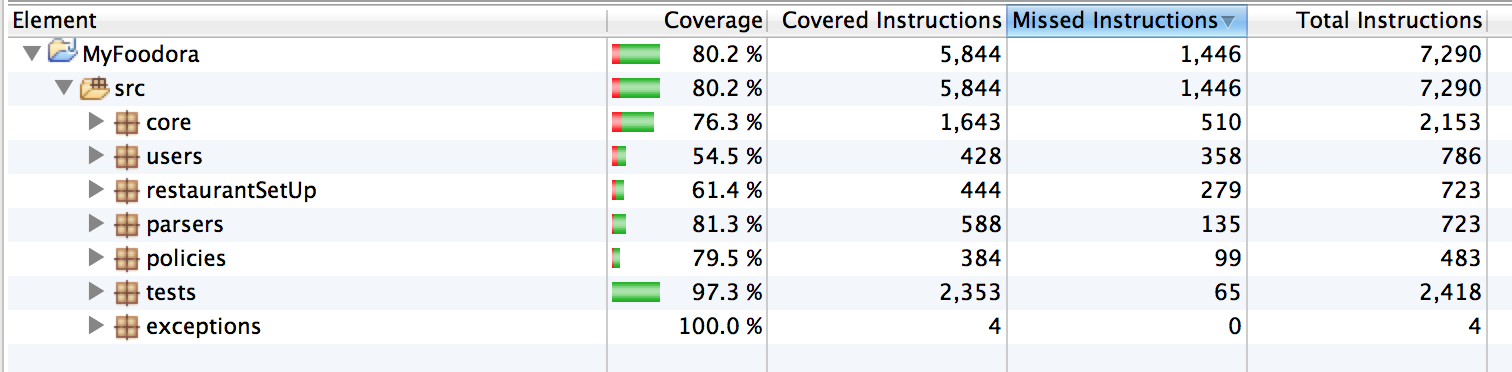
\includegraphics[scale=0.47]{./img/coverage_start.png} 
  \end{center}
  \caption{Code coverage results when using \textsc{EclEmma} for
  the first time.}
  \label{fig:coverage_first}
\end{figure} 

Next comes up the question to what extend the code has to be tested
while still being efficient.
It seems as ``\textit{the amount of testing necessary depends on a number of
factors}''~\cite{artimaHowMuchCoverage} that themselves depend
on how the code is written and what functions it implements.
Eventhough no particular goal for the coverage was set,
the plug-in allowed us to highlight the parts of the code that \emph{might not have been tested}
or that \emph{might be useless}. We finally achieved a $84.9\%$ code coverage after review (fig.~\ref{fig:coverage_end}). (--> @John UPDATE)

\begin{figure}[h]
  \begin{center}
    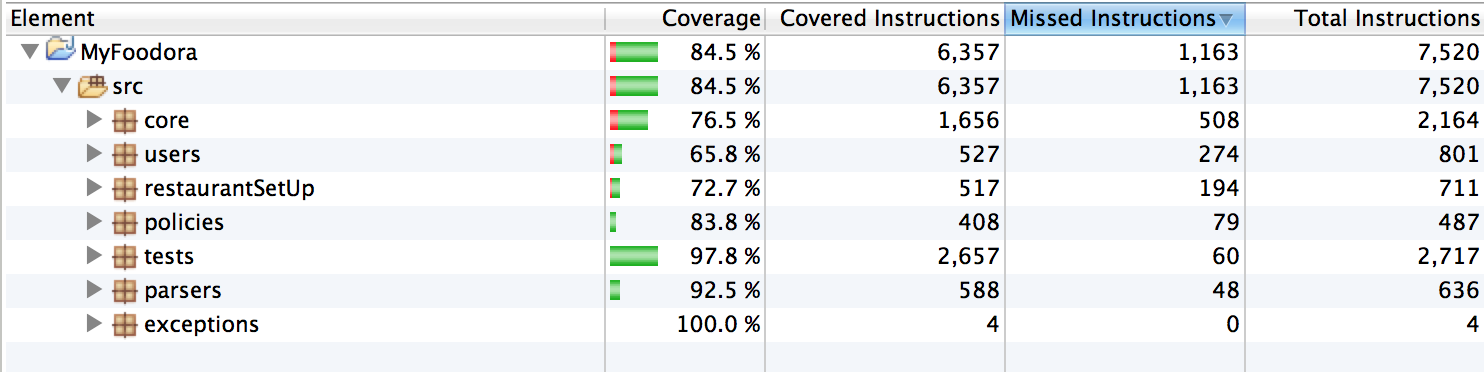
\includegraphics[scale=0.47]{./img/coverage_end.png} 
  \end{center}
  \caption{Code coverage results after review of
  tests using first results (fig.~\ref{fig:coverage_first}).}
  \label{fig:coverage_end}
\end{figure}

% section testing (end)